\documentclass{beamer}
\usepackage{amsthm}
\usepackage{xcolor}
\usepackage{amsmath}
\usepackage[absolute,overlay]{textpos}
\usetheme{Madrid}
\setbeamertemplate{navigation symbols}{}%remove navigation symbols
\useinnertheme{circles}
%Information to be included in the title page:
\title{Introduction to Nextflow
}

\graphicspath{{./figures/}}
\setbeamertemplate{itemize subitem}{\small$\circ$}
\author{Jakub Koubele}
\date{\today}

\renewcommand{\insertshortauthor}{Jakub Koubele}  
\renewcommand{\insertshorttitle}{Coding week 2026}
\renewcommand{\insertshortdate}{\today} % Define custom text for 3rd block


\usepackage{amsthm}
\newcommand*{\QED}{\hfill\ensuremath{\blacksquare}}
\begin{document}	
	
	\frame{\titlepage}	
	
\begin{frame}
	\frametitle{Nextflow is...}		
	
	\begin{textblock*}{3cm}(1cm,1.8cm)
		
\includegraphics[width=3cm]{nf_logo.png}
	\end{textblock*}
	
	\pause
	\begin{itemize}
		\item \textbf{workflow management system} used to organize and execute bioinformatics pipelines.
		\pause			
		\item \textbf{domain-specific language} (DSL) built on Groovy and running on the Java Virtual Machine (JVM).	
		\pause
		\item \textbf{powering nf-core}, a collection of high-quality, standardized bioinformatics pipelines.
	\end{itemize}	
	
	\only<4->{
		\begin{textblock*}{3cm}(1cm,6.4cm)
			
\includegraphics[width=3cm]{nf_core_logo.png}
		\end{textblock*}
	}
	
\end{frame}

\begin{frame}
	\frametitle{Why workflow management?}	
	
	Many bioinformatics pipelines face these challenges:
	\pause
	\begin{itemize}
		\item Using many \textbf{heterogeneous tools} (command-line programs, R/Python scripts, etc.) that must be ``glued'' together.
		\pause		
		\begin{itemize}	
			\item Different tools have different requirements — packages and environments need to be managed.
		\end{itemize}
		\pause
		
		\item \textbf{Data are big} $\to$ parallelization and/or execution on HPC is desired.
		
		\pause
		
	
	
	\item Pipelines form \textbf{dependency graphs} (not just step 1 $\to$ step 2 $\to$ step~3 etc.).
	\pause
	\begin{itemize}
		\item The execution order should be resolved automatically (tasks may finish asynchronously).
		\pause
		\item If part of the pipeline changes, re-run only affected downstream steps (caching).
	\end{itemize}
		
	\end{itemize}	
\end{frame}

\begin{frame}
	\frametitle{How Nextflow helps}
	
	\pause
	
	\begin{itemize}
		\item Language for ``gluing'' tools into pipelines. Basic components: \textbf{processes} and \textbf{channels}.
		\begin{itemize}
			\item \textbf{Processes}: define computational tasks (scripts, command-line tools, etc.).
			\item \textbf{Channels}: transport data between processes (in asynchronous queues).
		\end{itemize}
	\pause
	\item Supports software environments: processes can run in containers (Docker, Singularity, etc.) or environments (Conda, modules, etc.).
	\pause
	\item Channels are asynchronous $\to$ automatic parallelization and flexible execution order.
	
	\pause
	\item Pipeline logic is separated from execution $\to$ easy deployment on HPC or cloud infrastructure.
	\end{itemize}

	
\end{frame}
	
	
\begin{frame}
	\frametitle{Pipelines as DAGs}
	
	\begin{itemize}
		\item Computational pipelines can be represented as \textbf{directed acyclic graphs (DAGs)}.
		\pause
		\begin{itemize}
			\item \textbf{Nodes}: represent data or intermediate results.
			\item \textbf{Edges}: represent dependencies between nodes; a child node is computed from the data in its parent nodes.
		\end{itemize}
	\end{itemize}
	\pause
	\begin{center}
		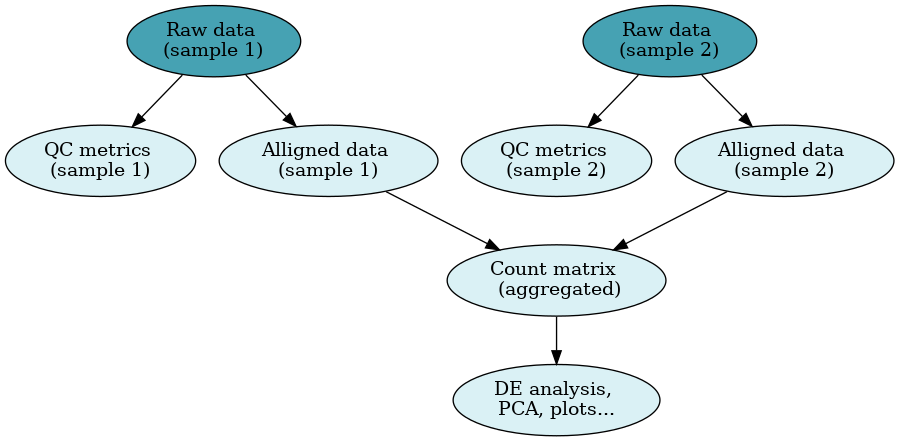
\includegraphics[width=11cm]{pipeline_dag.png}
	\end{center}
	
\end{frame}
	
	
	
	
\end{document}